\begin{figure}
  \begin{center}
    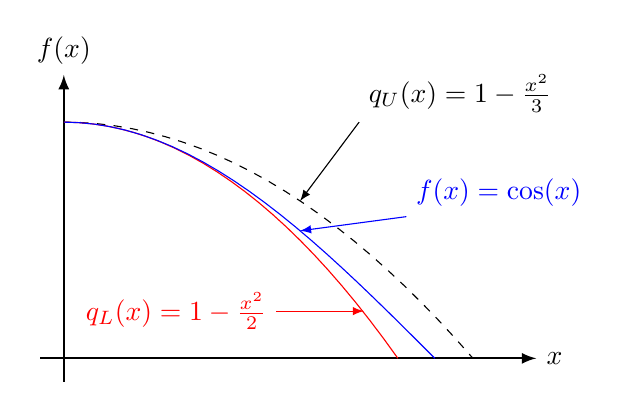
\begin{tikzpicture}[>=latex,xscale=3.0,yscale=3.0]
      \draw[thick,->] (-0.1,0) -- (2,0) node[right] {$x$};
      \draw[thick,->] (0,-0.1) -- (0,1.2) node[above] {$f(x)$};
      \draw[dashed,domain=0:sqrt(3)]   plot (\x,{1-(\x^2)/3.0});
      \draw[red,domain=0:sqrt(2)]   plot (\x,{1-0.5*\x^2});
      \draw[blue,domain=0:pi/2]   plot (\x,{cos(\x r )}) ;
      \draw[->](1.25,1)node[above right] {$q_U(x) = 1-\frac{x^2}{3}$}--(1,0.666);

      \draw[->,blue](1.45,0.6)node[above right] {$f(x) = \cos(x)$}--(1,0.54);

      \draw[->,red] (0.9,0.2)node[left]{$q_L(x) =1-\frac{x^2}{2}$}--(1.27,0.2);
    \end{tikzpicture}
  \end{center}
\caption{Upper and lower polynomial bounds for $\cos(x)$, $x \in ( 0, \tfrac\pi2]$.}
\label{fig:upper-lower-bnounds}
\end{figure}